\chapter{代数拓扑}
    \section{Brouwer不动点定理与Sperner引理}
    我们首先叙述 Brouwer不动点定理与Sperner引理:
    \begin{theorem}[Brouwer不动点定理]
        设 $f$ 是 $n$ 维闭球 $B^n$ 到自身的连续映射, 则 $f$ 必有不动点.
    \end{theorem}
    \begin{lemma}[Sperner引理]
        设 $K=[v_0,\dots,v_n]$ 是 $n$ 维单纯形, 考虑其三角剖分 $T$, 将 $T$ 的顶点 $(n+1)$ 染色, 即定义 $\lambda:V(T)\rightarrow\{0,\dots,n\}$, 且满足对任意指标子集
        $\{i_0,\dots,i_k\}\subseteq\{0,\dots,n\}$, $\lambda$ 在 $[v_{i_1},\dots,v_{i_k}]$ 上的限制的值域包含于 $\{i_1,\dots,i_k\}$. 则一定存在 $u_0,\dots,u_n\in V(T)$, 
        使得 $[u_0,\dots,u_n]$ 是三角剖分 $T$ 的单形, 且 $\lambda(u_i)$ 互不相同.
        \begin{figure}[hbtp]
            \centering
            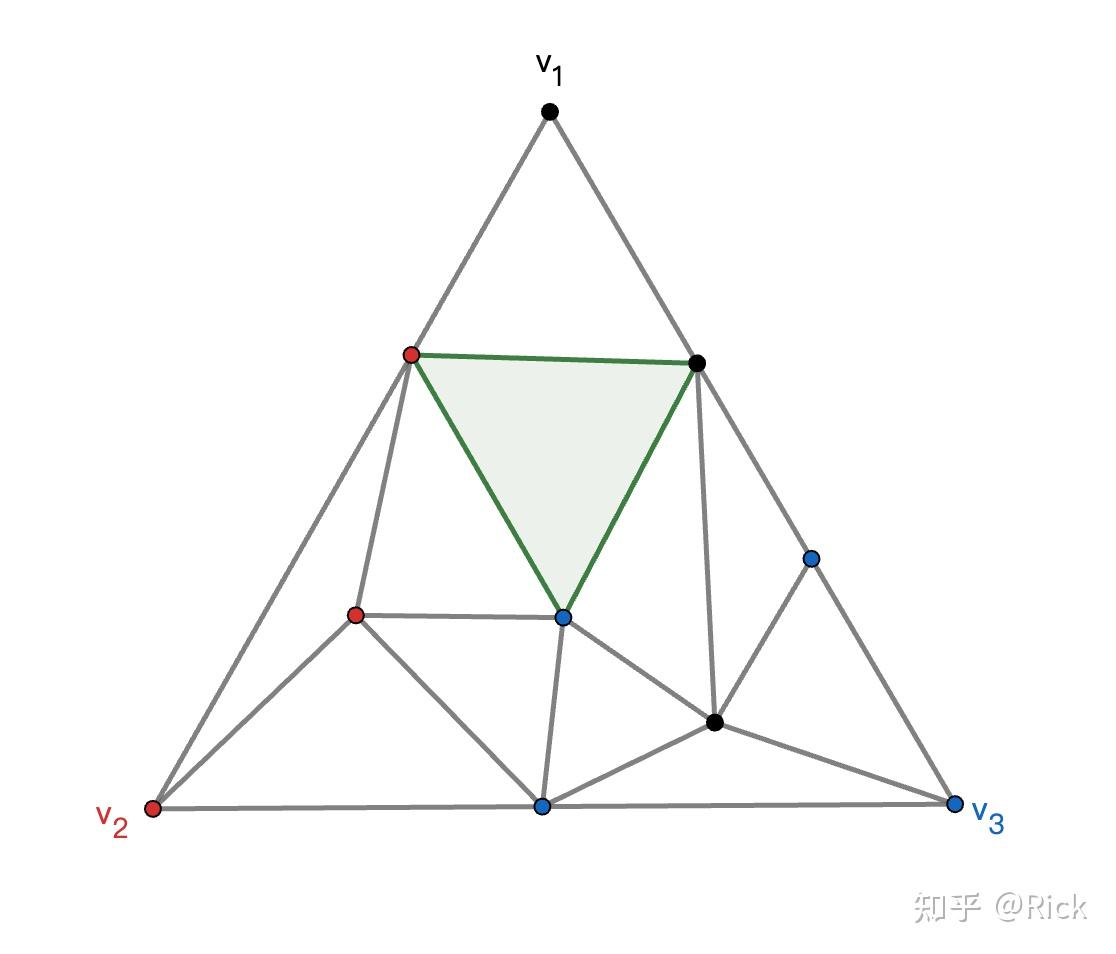
\includegraphics[scale=0.2]{Figures/SpernerLemma.jpg}
            \caption[SpernerLemma]{Sperner引理示意图}
        \end{figure}
    \end{lemma}

    它们一个是拓扑的定理, 一个是组合的定理, 看似没有联系, 但实际上我们能证明它们是等价的: 由于 $B^n\cong K$, 我们将 Brouwer不动点定理的叙述改为 $K$ 到自身的连续映射 $f$ 必有不动点.

    $1^{\circ}$:Sperner引理 $\Rightarrow$ Brouwer不动点定理

    
